%%%%%%%%%%%%%%%%%%%%%%%%%%%%%%%%%%%%%%%%%%%%%%%%%%%%%%%%%%%%%%%%%%%%%%%
%% Related Work
\subsection{ROS: Robotic Operating System}
\label{sec:basic-ros}
    
Das Robotic Operating System, kurz ROS, ist ein Middleware-Framework zur Steuerung und Verwaltung von Personal-Robotern. Es verwendet eine Paket und Node Struktur um einzelne Aktoren und Sensoren einzelner Robotersystem zu betreiben. Das ROS dient dabei als Abstraktionsebene für die Entwickler und versucht die Anwendungsebene von der Hardwareebene zu trennen. Das Framework wird am Robotikinstitut Willow Garage in Zusammenarbeit mit der Open Source Robotics Foundation entwickelt, stammt aber ursprünglich vom Stanford Artificial Intelligence Laboratory. Dort wurde 2007 im Rahmen des Stanford-AI-Robot-Projektes die Entwicklung aufgenommen. ROS ermöglicht während der Entwicklung und des Betriebs ein Cross-Plattform System, da es kompatible Versionen für Windows (experimentell), Linux und Mac OS X gibt. Außerdem steht ein Multi(programmier)sprachen System zur Verfügung. So ist es möglich eigene Nodes mit C++, Python oder Java zu entwickeln.\cite{quigley2009ros} Neben den Standardkonzepten und -paketen gibt es eine Community, die eigene Pakete auf der ROS-Homepage zur Verfügung stellt. Die folgenden Abschnitte erläutern die ROS-Kernkonzepte, welche für die Entwicklung eingesetzt wurden.

\subsubsection{Package und Nodes}

\textit{Packages} dienen der strukturellen Verwaltung aller Dateien im ROS-System. Nodes, Launch-Files, Services, Actions und Messages sind immer an ihr Paket gebunden und können nur unter deren Namen erreicht werden. Für die Verlinkung und die Erreichbarkeit gebauter Pakete ist das ROS-interne Buildsystem \textit{Catkin} zuständig. Es benötigt ebenfalls den \textbf{eindeutigen} Package-Namen für den Build und Verwaltungsprozess. Neben den ROS bezogenen Daten können in einem Paket aber auch ROS unabhängige APIs angelegt und verwaltet werden. So werden unter anderem einzelne Pakete für Treiber genutzt. Ein ROS Paket folgt dem "Goldilocks" Prinzip: Genug Funktionalität um nützlich zu sein, aber nicht zu viel, damit die Verwendbarkeit nicht zu komplex wird. Der Aufbau eines ROS Pakets findet sich in Anhang \ref{app:rosp}

Neben der strukturellen Verteilung gibt es auch die Funktionale Trennung. Dies wird durch einzelne \textit{Nodes} erreicht. Jeder Node hat einen bestimmten Aufgabenbereich. Erst das Zusammenspiel mehrerer Nodes ergibt ein Robotersystem. So ist ein Node zum Beispiel für die Berechnung der Inversen Kinematik zuständig, ein anderer für die Lokalisierung des Roboters im Raum und ein dritter für das User-Interface. Diese Verteilung der Funktionalitäten hat mehrere Vorteile. Da jeder Node in einem eigenen Prozess gestartet wird ist das komplette System robuster. Jeder Node muss so entwickelt werden, dass er eigenständig weiterlaufen kann, auch wenn ein benötigter Node durch einen Fehler abgestürzt ist. Jeder Node wird mit einem System weit einmaligen Namen aufgerufen unter dem er vom System erreicht und angezeigt werden kann. Nodes kommunizieren untereinander mit Hilfe von Topics (siehe \ref{sec:basic-ros-topics}).Soll ein ROS Node gestartet werden kann dieser mit Hilfe des ROS-Befehls aufgerufen werden:

\begin{lstlisting}[language=bash]
rosrun <paket-name> <nodetype-name>
\end{lstlisting}

Der Paketname und der Nodetype sind erfordliche Felder. Darüber hinaus können Parameter angegeben werden die für den Node notwendig sind. Eine weitere Möglichkeit einen und mehrere Nodes zu starten ist ein Launchfile (siehe Anhang \ref{app:roslaunch}). In diesem können Nodes, Parameter und Argumente aufgelistet werden. Zu beachten ist jedoch, dass die Nodes in einer zufälligen Reihenfolge gestartet werden. Ein Launch-File kann mit folgendem Befehl gestartet werden:

\begin{lstlisting}[language=bash]
roslaunch <paket-name> <launchfile-name>
\end{lstlisting}

Damit ein Node gestartet werden kann muss vorher ein ROS-Master aktiv sein, mit dem sich der Node verbinden kann. Ist der Node verbunden kann er auf die Topics, Services, Actions und den Parameter Server des Master zugreifen.

\subsubsection{Master und Parameter Server}
Der ROS Master ist ein zentraler Dienst für ganze System. Er beinhaltet einen Namen- und Registrierungs-Service an dem sich andere Nodes, auch Services, anmelden können. Der Master wird benötigt, damit die Nodes sich gegenseitig im System verbinden können. Der Nachrichten Transport geht nicht direkt über den Master er verbindet nur die beiden Nodes, welche anschließend via einer Peer-to-Peer Verbindung kommunizieren.

 \begin{figure}[h]
 	\centering
 	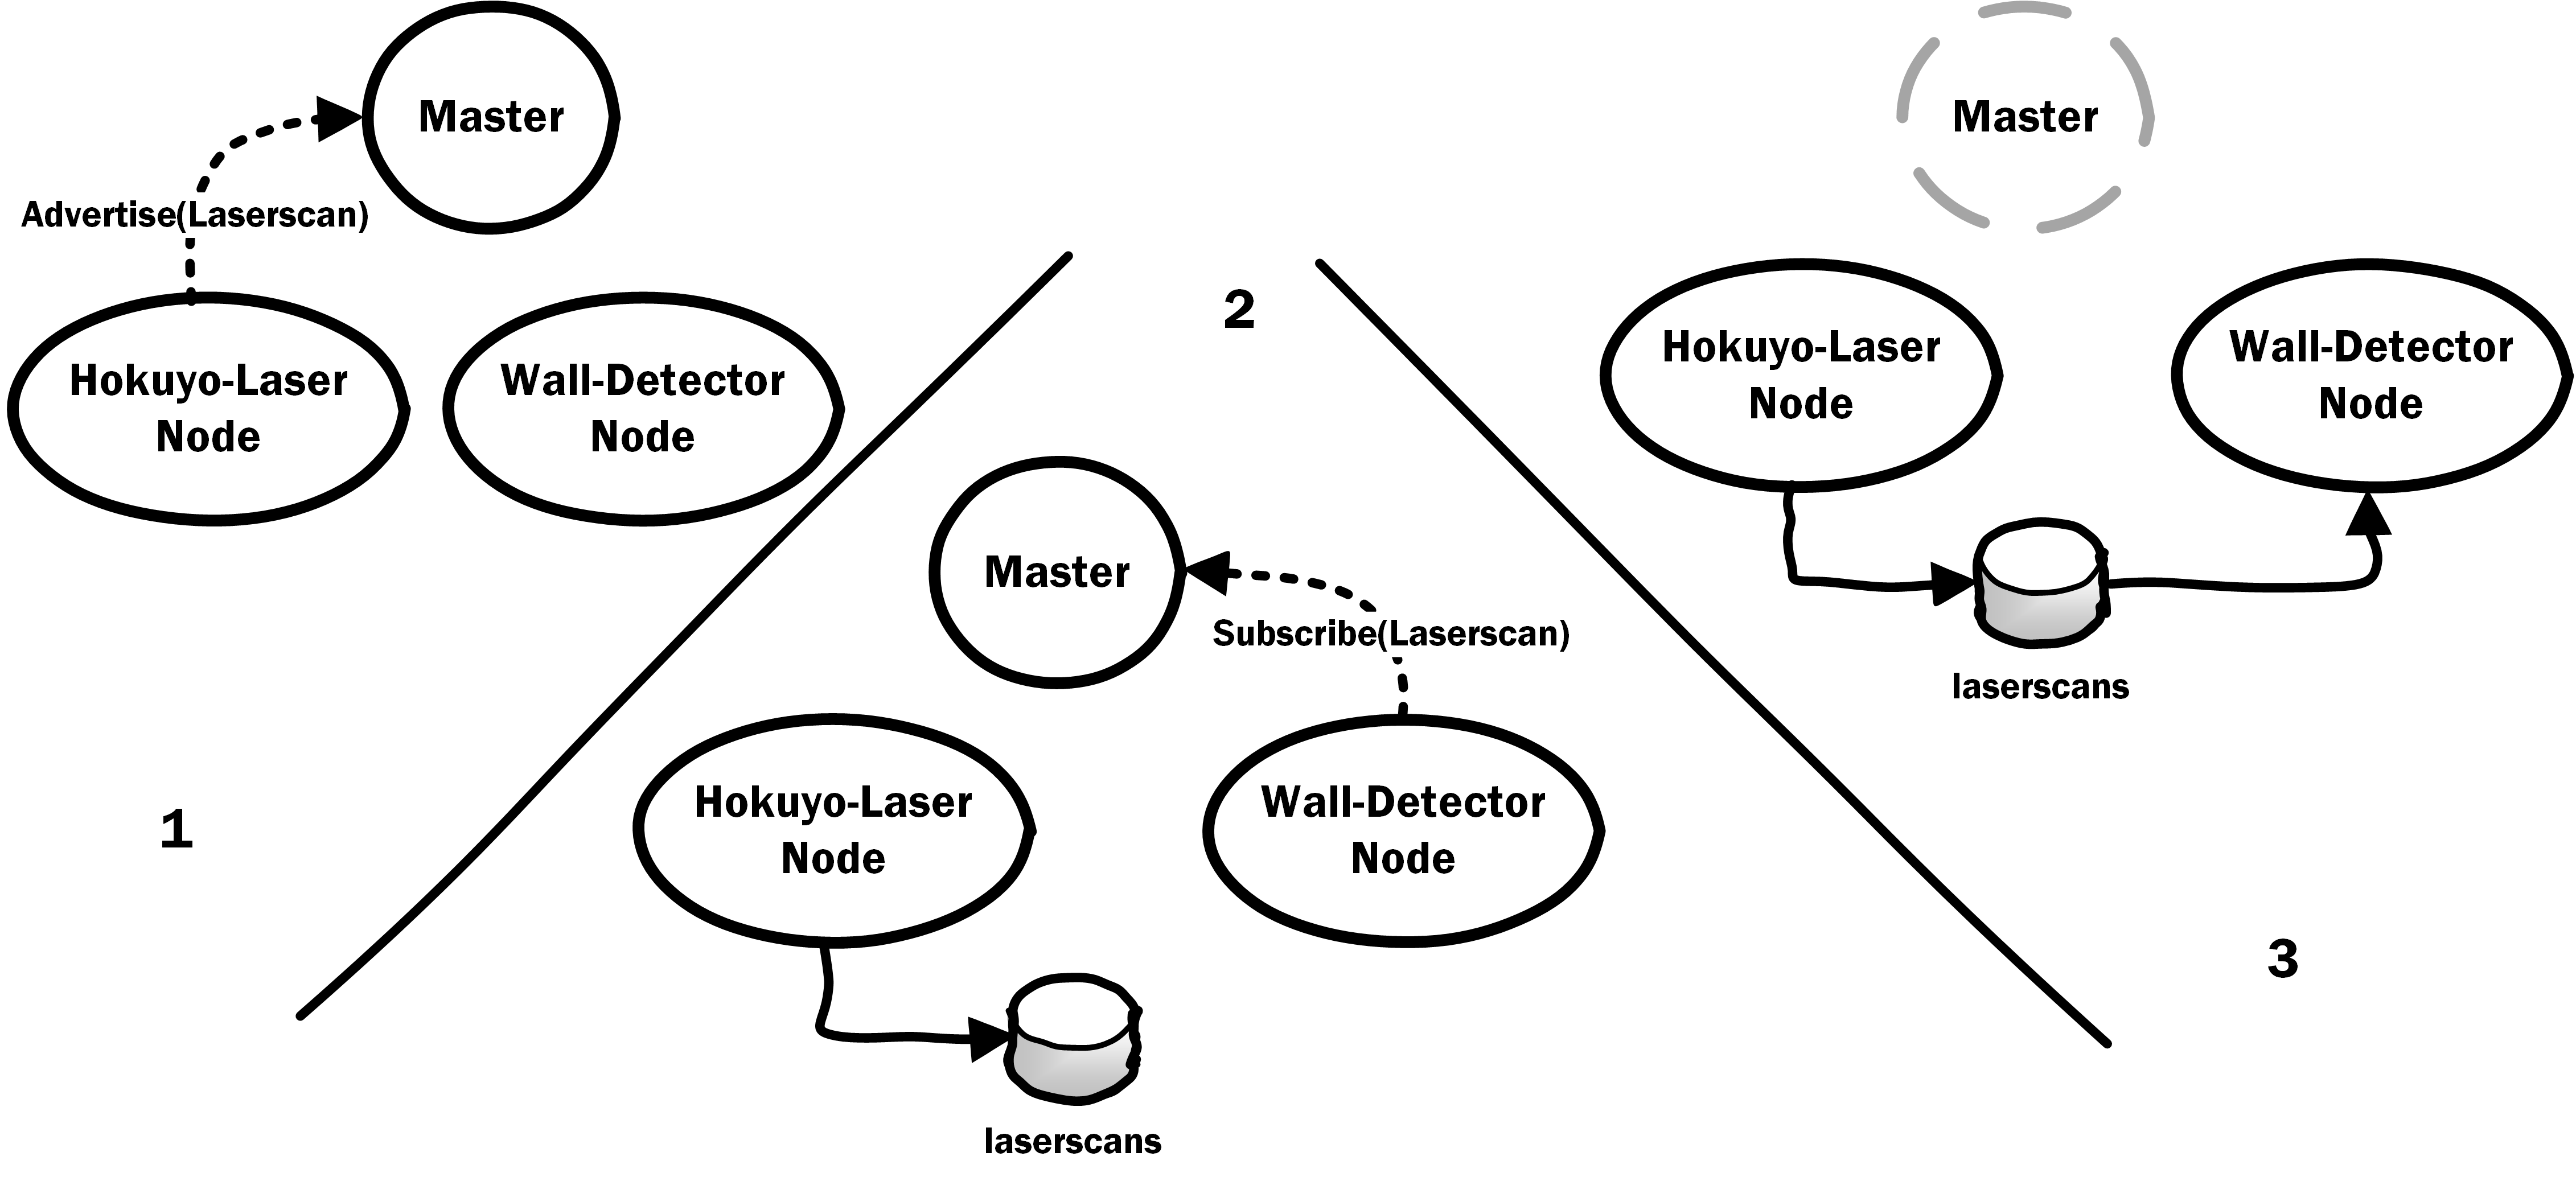
\includegraphics[scale=0.8]{fig/masternode}   
 	\caption[Master Service]{Master Service: (1) Der Hokuyo Laser Node meldet sich beim Master an, das er Laserscans zur Verfügung stellt. (2) Der Laser Node stellt seine Daten zur Verfügung und der Wall Detector meldet sich beim Master, dass er Laserscans benötigt. Der Master stellt die Verbingunsinformationen bereit und zieht sich dann zurück (graue Markierung). (3) Die Verbindung zwischen Laser Node und Detector Node ist hergestellt.}
 	\label{fig:basic-ros-masternode}
 \end{figure}
 
 Dieses Verfahren reduziert die Netzwerklast stark im Vergleich zu einem Broadcasting-Verfahren. Tests zeigten, dass ein Kamera-Node (openni) ein Netzwerk mit seinen 3D-Punktwolken vollständig auslastet. Dabei wurde die Punktwolke auf der physikalischen Maschine eins erzeugt und auf eine zweite Maschine via WLAN übertragen. Die Delay-Zeit der Wolken war dabei sehr hoch > 1 Sekunde und wurde, je länger die Übertragung dauerte höher. Werden die Daten jedoch auf der Maschine vor verarbeitet und nur noch die wichtigen Daten übertragen, sowie die Übertragungsrate reduziert, ist die Übertragung der Daten unkritisch. Nun gehen nur noch die Verbindungsdaten zwischen Nodes und Master über das Netzwerk und die reduzierte Datenmenge.
 
 \begin{figure}[h]
 	\centering
 	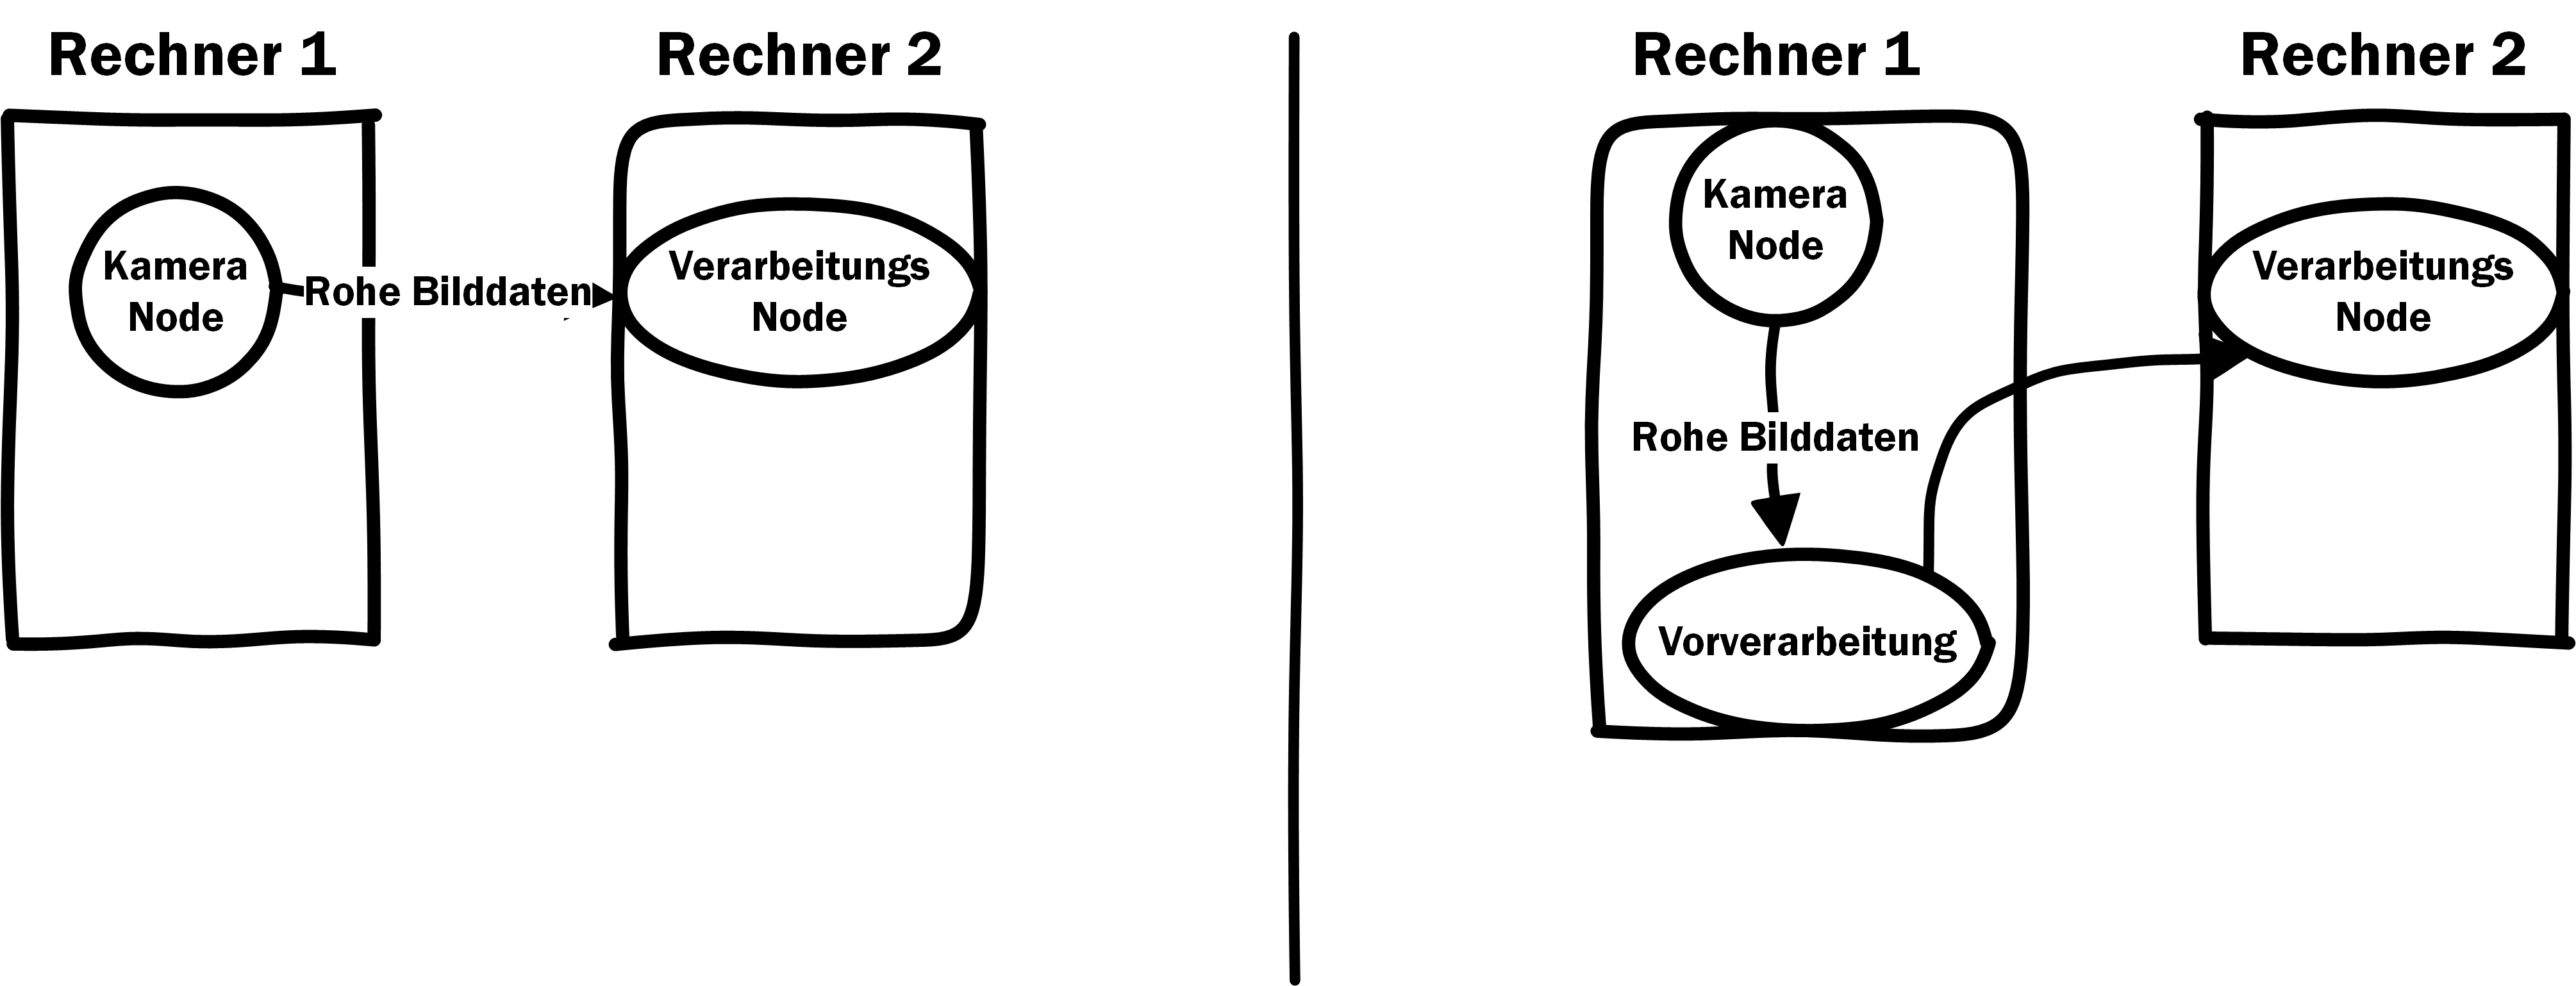
\includegraphics[scale=0.8]{fig/masternet}   
 	\caption[Netzwerk Entlastung durch Peer-to-Peer Verbindungen]{Netzwerk Entlastung durch Peer-to-Peer Verbindungen. Links: Ohne Datenvorverarbeitung, Rechts: Mit Datenvorverarbeitung}
 	\label{fig:basic-ros-masternet}
 \end{figure}
 
 Neben dem Namen-Service verwaltet der ROS Master auch den Parameter Server. Dieser besteht aus einem Dictonary, einer großen Key-Value-Map, welches global erreicht werden können. Nodes haben so die Möglichkeit vordefinierte Daten ab zugreifen oder selber welche zu schreiben. So können Sensoren oder Aktoren kalibriert und konfiguriert werden. Der Zugriff auf diese Daten hat keine hohe Performance. Er ist für einen statischen Zugriff gedacht und kann mit einer Baum-Struktur geordnet werden, so lassen sich zusammenhängende Daten mit einer Abfrage am Server abrufen.

\subsubsection{Topics und Messages}
\label{sec:basic-ros-topics}

ROS bietet für die Kommunikation zwischen Nodes ein \textit{Topic}-System. Jeder Topic entspricht dabei einem benannten Bus, auf welchen anonyme \textit{Publisher} und \textit{Subscriber} zugreifen können. Die Daten können dabei als TCP-Pakete (TCPROS) oder als UDP-Pakete(UDPROS) gesendet werden. Ein Topic besitzt einen eindeutigen Namen im System und einen eindeutigen Typen, der anhand des übersendeten Message-Typen definiert wird. Jede Topic kann nur einen Message-Typen versenden. Dieser Type ist nicht im Master bekannt, jedoch können sich Subscriber nur mit dem entsprechenden Typen anbinden. Die Anzahl der Subscriber und Publisher für einen Topic ist nur durch die Systemleistung beschränkt.

\begin{figure}[h]
	\centering
	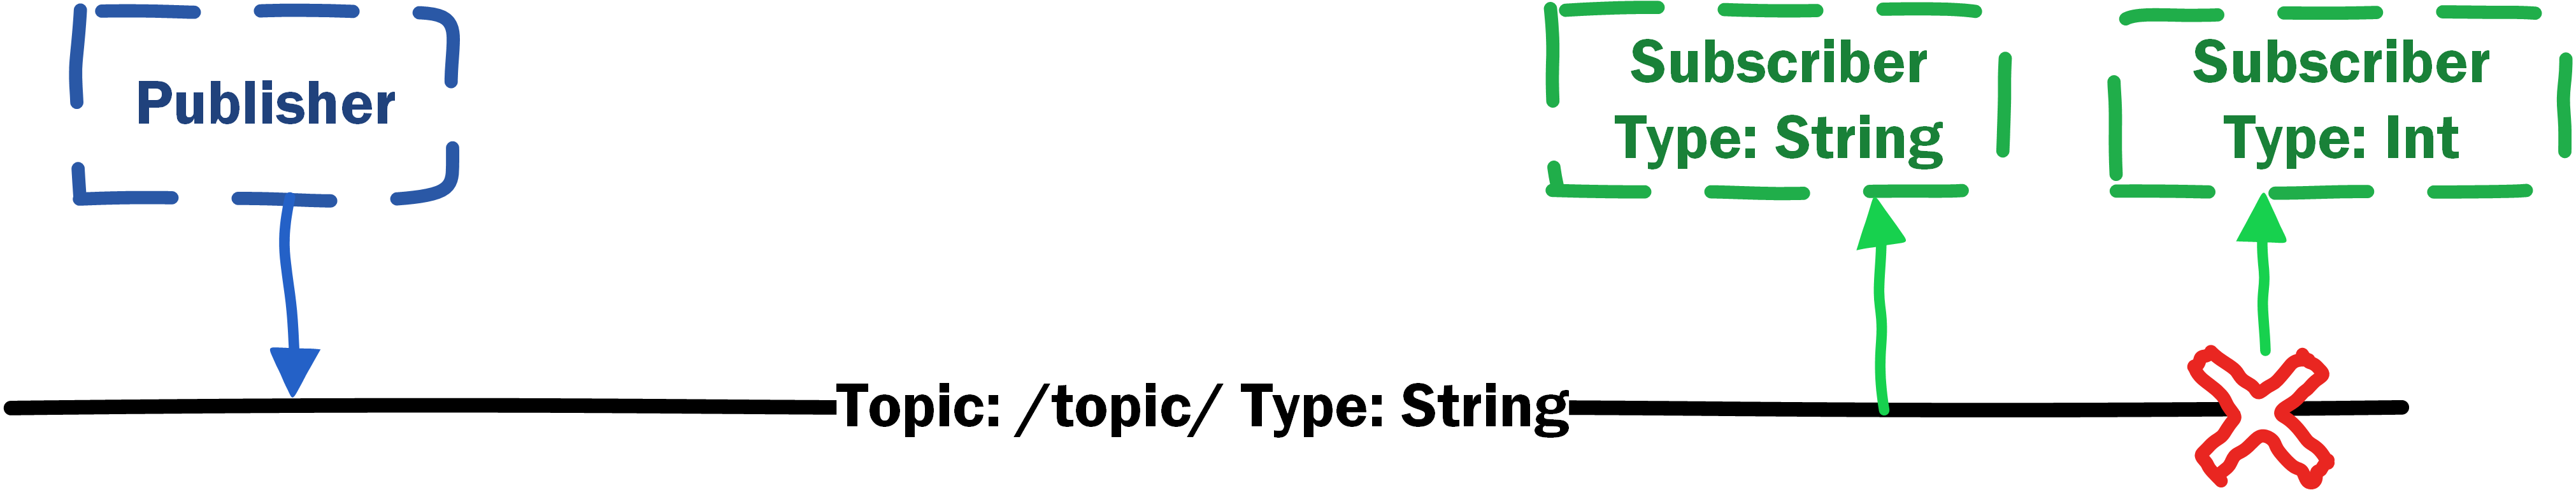
\includegraphics[scale=0.8]{fig/topic}   
	\caption[Topic Beispiel]{Beispiel für eine Topic mit dem Namen /topic und dem Type String. Ein Publisher schreibt Daten in den Bus, ein Subscriber liest diese aus. Die Verbindung eines zweiten Subscribers schlägt auf Grund des falschen Types fehl.}
	\label{fig:basic-ros-topic}
\end{figure}

Publisher veröffentlichen ihre Daten in den Bus und haben nur einen schreibenden Zugriff. Sie bekommen kein Feedback an wen die Daten gesendet worden sind oder ob die Daten überhaupt empfangen worden sind. Der erste Publisher, der sich auf einem Topic verbindet gibt den Typen vor.

Subscriber lesen die Daten vom Bus und geben sie für die Weiterverarbeitung weiter. Sie bekommen normalerweise keine Informationen über den Absender der Daten. Subscriber können sich nur bei einem Topic registrieren, wenn der Message-Type stimmt.

Subscriber und Publisher haben jeweils eigene Cache-Systeme die Nachrichten vor- oder zurückhalten können. Ein Topic ist ein einfachgerichteter Streaming-Dienst ist. Da in einem Roboter-System auch Remote Procedure Calls benötigt werden, um zum Beispiel Antworten auf Anfragen zu erhalten oder synchronisierte Aufgaben zu erledigen, wurde das Service-Paket als weiteres Kernkonzept angelegt.

\subsubsection{Services}

\textit{Services} ermöglichen es einen Remote Procedure Call Node übergreifend durchzuführen. Dazu muss Node A seinen Service am Master registriert haben und einen Service Server gestartet haben. Node B kann nun mit einem Service Client auf den registrierten Service zugreifen und eine Anfragen starten. Während die Anfrage verarbeitet wird, kann Node B nun je nach Anforderung blockieren oder weiter arbeiten. Node A verarbeitet nun die Anfrage und antwortet Node B mit dem Ergebnis. Der Service selbst, sowie die Parameter und die Rückgabewerte, sind für jeden Service eindeutig und werden vorher via zwei Messages, eine für die Request und eine für die Response, festgelegt. Analog zu den Topics werden Services am Master mit einem eindeutigen Namen angemeldet unter dem sie erreichbar sind. Dies ermöglicht auch einen einfachen Austausch von verschiedenen Implementierungen.

\subsubsection{Action-Lib}
Ein aktiver Service schickt erst eine Rückmeldung an den Aufrufer, wenn er seine Aufgabe erledigt hat. Um auch einen Zwischenstand schicken zu können wurde die Actionlib eingeführt. Dieses Paket ist eigentlich keine Entwicklung der ROS-Entwickler sondern ein Community-Package. Inzwischen wurde es aber von der OSR-Foundation übernommen und als eins der Kernkonzepte eingestuft.

Analog zu den Services besitzt auch die Action-Lib einen Server- und einen Client Teil. Der Client fordert vom Server eine Aktion an, dabei übergibt er ein \textit{Goal}. Dieses beinhaltet die benötigten Parameter für den Server. Der Server arbeitet die Anfrage ab, dabei kann er auch \textit{Feedback}, Zwischenstände, zurückschicken. Ist die Anfrage abgearbeitet schickt der Server ein \textit{Result} an den Client zurück. Wie auch beim Service ist die Art der Aktion eindeutig. Die Anzahl der Parameter bei Goal, Feedback und Result sind fest definiert und können zur Laufzeit nicht geändert werden.